% \documentclass[journal = esthag, manuscript = article]{achemso}

\documentclass[letterpaper,12pt,oneside]{article}\usepackage[]{graphicx}\usepackage[]{color}
%% maxwidth is the original width if it is less than linewidth
%% otherwise use linewidth (to make sure the graphics do not exceed the margin)
\makeatletter
\def\maxwidth{ %
  \ifdim\Gin@nat@width>\linewidth
    \linewidth
  \else
    \Gin@nat@width
  \fi
}
\makeatother

\definecolor{fgcolor}{rgb}{0.345, 0.345, 0.345}
\newcommand{\hlnum}[1]{\textcolor[rgb]{0.686,0.059,0.569}{#1}}%
\newcommand{\hlstr}[1]{\textcolor[rgb]{0.192,0.494,0.8}{#1}}%
\newcommand{\hlcom}[1]{\textcolor[rgb]{0.678,0.584,0.686}{\textit{#1}}}%
\newcommand{\hlopt}[1]{\textcolor[rgb]{0,0,0}{#1}}%
\newcommand{\hlstd}[1]{\textcolor[rgb]{0.345,0.345,0.345}{#1}}%
\newcommand{\hlkwa}[1]{\textcolor[rgb]{0.161,0.373,0.58}{\textbf{#1}}}%
\newcommand{\hlkwb}[1]{\textcolor[rgb]{0.69,0.353,0.396}{#1}}%
\newcommand{\hlkwc}[1]{\textcolor[rgb]{0.333,0.667,0.333}{#1}}%
\newcommand{\hlkwd}[1]{\textcolor[rgb]{0.737,0.353,0.396}{\textbf{#1}}}%
\let\hlipl\hlkwb

\usepackage{framed}
\makeatletter
\newenvironment{kframe}{%
 \def\at@end@of@kframe{}%
 \ifinner\ifhmode%
  \def\at@end@of@kframe{\end{minipage}}%
  \begin{minipage}{\columnwidth}%
 \fi\fi%
 \def\FrameCommand##1{\hskip\@totalleftmargin \hskip-\fboxsep
 \colorbox{shadecolor}{##1}\hskip-\fboxsep
     % There is no \\@totalrightmargin, so:
     \hskip-\linewidth \hskip-\@totalleftmargin \hskip\columnwidth}%
 \MakeFramed {\advance\hsize-\width
   \@totalleftmargin\z@ \linewidth\hsize
   \@setminipage}}%
 {\par\unskip\endMakeFramed%
 \at@end@of@kframe}
\makeatother

\definecolor{shadecolor}{rgb}{.97, .97, .97}
\definecolor{messagecolor}{rgb}{0, 0, 0}
\definecolor{warningcolor}{rgb}{1, 0, 1}
\definecolor{errorcolor}{rgb}{1, 0, 0}
\newenvironment{knitrout}{}{} % an empty environment to be redefined in TeX

\usepackage{alltt}
\usepackage[paperwidth=8.5in,paperheight=11in,top=1in,bottom=1in,left=1in,right=1in]{geometry}
\usepackage[T1]{fontenc}
\usepackage[colorlinks  =true, allcolors=Blue]{hyperref}
\usepackage[usenames,dvipsnames]{xcolor}
\usepackage{lineno}
\usepackage{cleveref}
\usepackage{acronym}
\usepackage{paralist}
\usepackage{setspace}
\usepackage{fancyhdr}
\pagestyle{fancy}
\fancyfoot[c]{S\thepage}
% \usepackage{showlabels}

% cleveref options
\crefname{table}{Table}{Tables}
\crefname{figure}{Figure}{Figures}
\renewcommand{\figurename}{Figure}

\renewcommand{\headrulewidth}{0pt}

%acronyms
\acrodef{chla}[chl-\textit{a}]{chlorophyll \textit{a}}
\acrodef{din}[DIN]{dissolved inorganic nitrogen}
\acrodef{emp}[EMP]{Environmental Monitoring Program}
\acrodef{iep}[IEP]{Interagency Ecological Program}
\acrodef{jas}[JAS]{July-August-September}
\acrodef{sfe}[SFE]{San Francisco Estuary}
\acrodef{wrtds}[WRTDS]{Weighted Regressions on Time, Discharge, and Season}
\acrodef{wwtp}[WWTP]{wastewater treatment plant}
\acrodefplural{wwtp}[WWTPs]{wastewater treatment plants}

%for supplemental figures/tables
\newcommand{\beginsupplement}{%
        \setcounter{table}{0}
        \renewcommand{\thetable}{S\arabic{table}}%
        \setcounter{figure}{0}
        \renewcommand{\thefigure}{S\arabic{figure}}%
     }

% for unit macros
\newcommand{\mgl}{mg L$^{-1}$}
\newcommand{\mugl}{$\mu$g L$^{-1}$}

%knitr options


\IfFileExists{upquote.sty}{\usepackage{upquote}}{}
\begin{document}

% supplementary material
\section*{Supplementary Information}

\noindent{\bf Four decades of water quality change in the upper San Francisco Estuary}
\vspace{0.1in}

\noindent Marcus W. Beck (beck.marcus@epa.gov), Thomas W. Jabusch,Philip R. Trowbridge, David B. Senn
\vspace{0.1in}

\beginsupplement

\noindent The following files are available free of charge: \cref{fig:trndcomp2,fig:trndcomp3,fig:stock}, \cref{tab:trndsann,tab:trndsbef,tab:trndsaft}

\begin{figure}
\centering
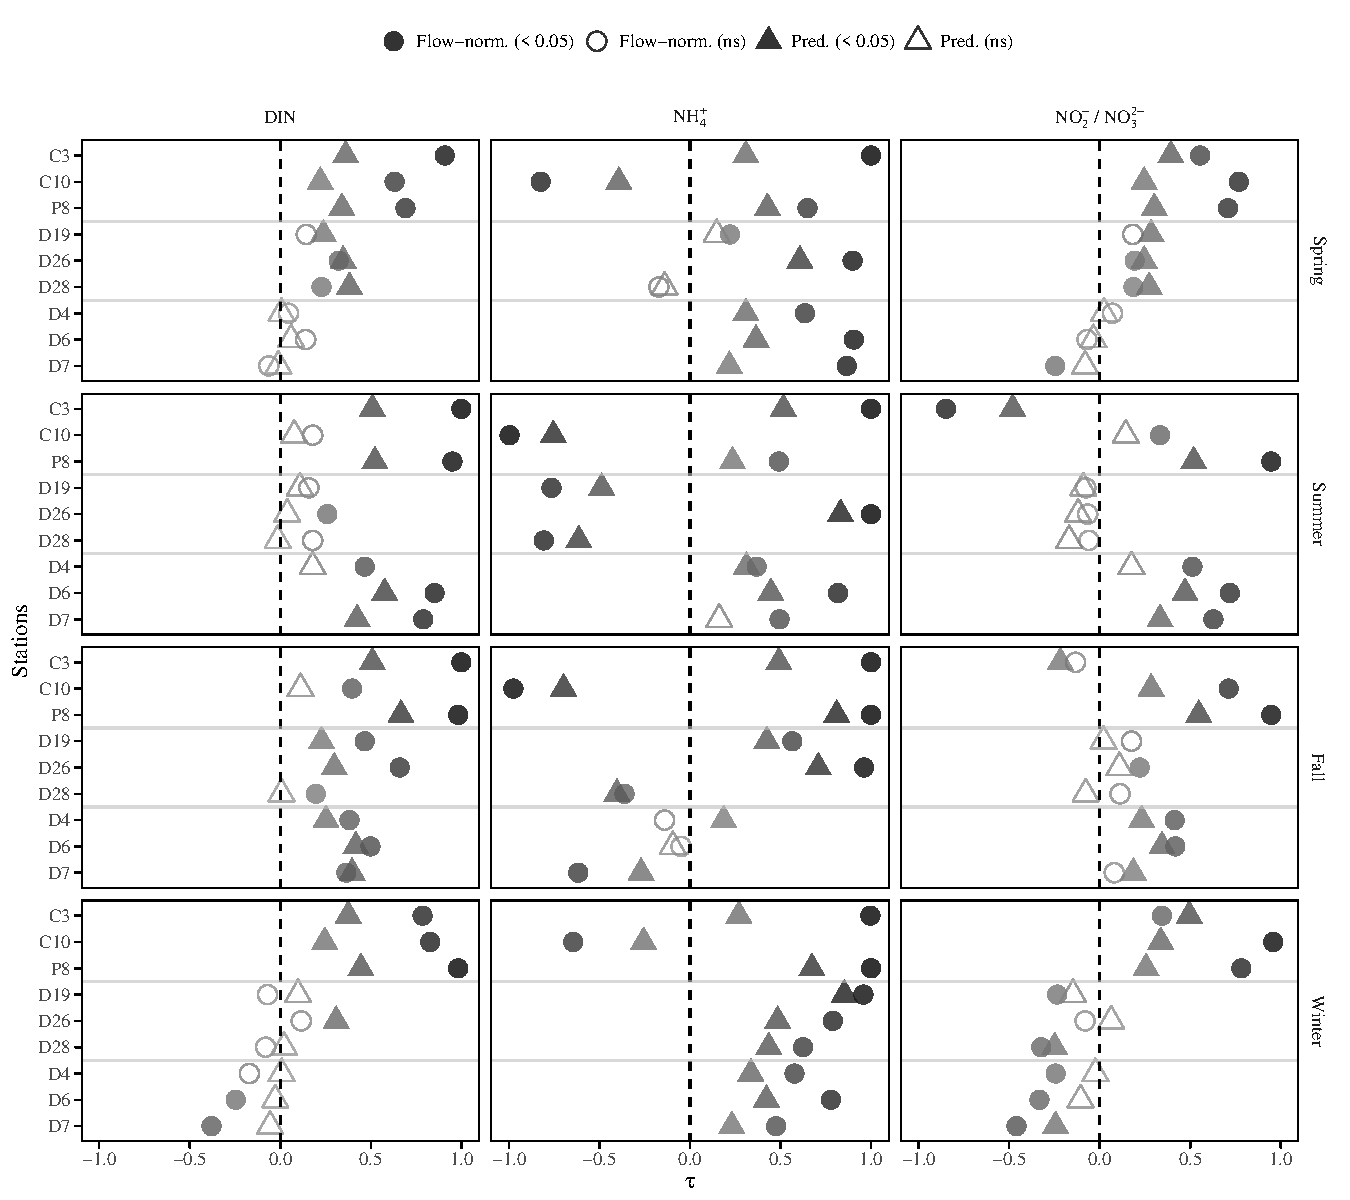
\includegraphics[width=1\textwidth,page=1]{figs/trndcomp2.pdf}
\caption{Results from seasonal Kendall tests on observed data (triangles) and flow-normalized predictions (circles) from \ac{wrtds} for nitrogen analytes. Results are shown as the percent change per year as the estimated Theil-Sen slope divided by the median for a given aggregation period (significance evaluated at $\alpha = 0.05$, based on $\tau$). Trends are shown separately for different seasonal groupings from 1976-1995. Months for each season are Spring: MAM, Summer: JJA, Fall: SON, Winter: DJF. See Figure 3 for annual comparisons.}
\label{fig:trndcomp2}   
\end{figure}

\begin{figure}
\centering
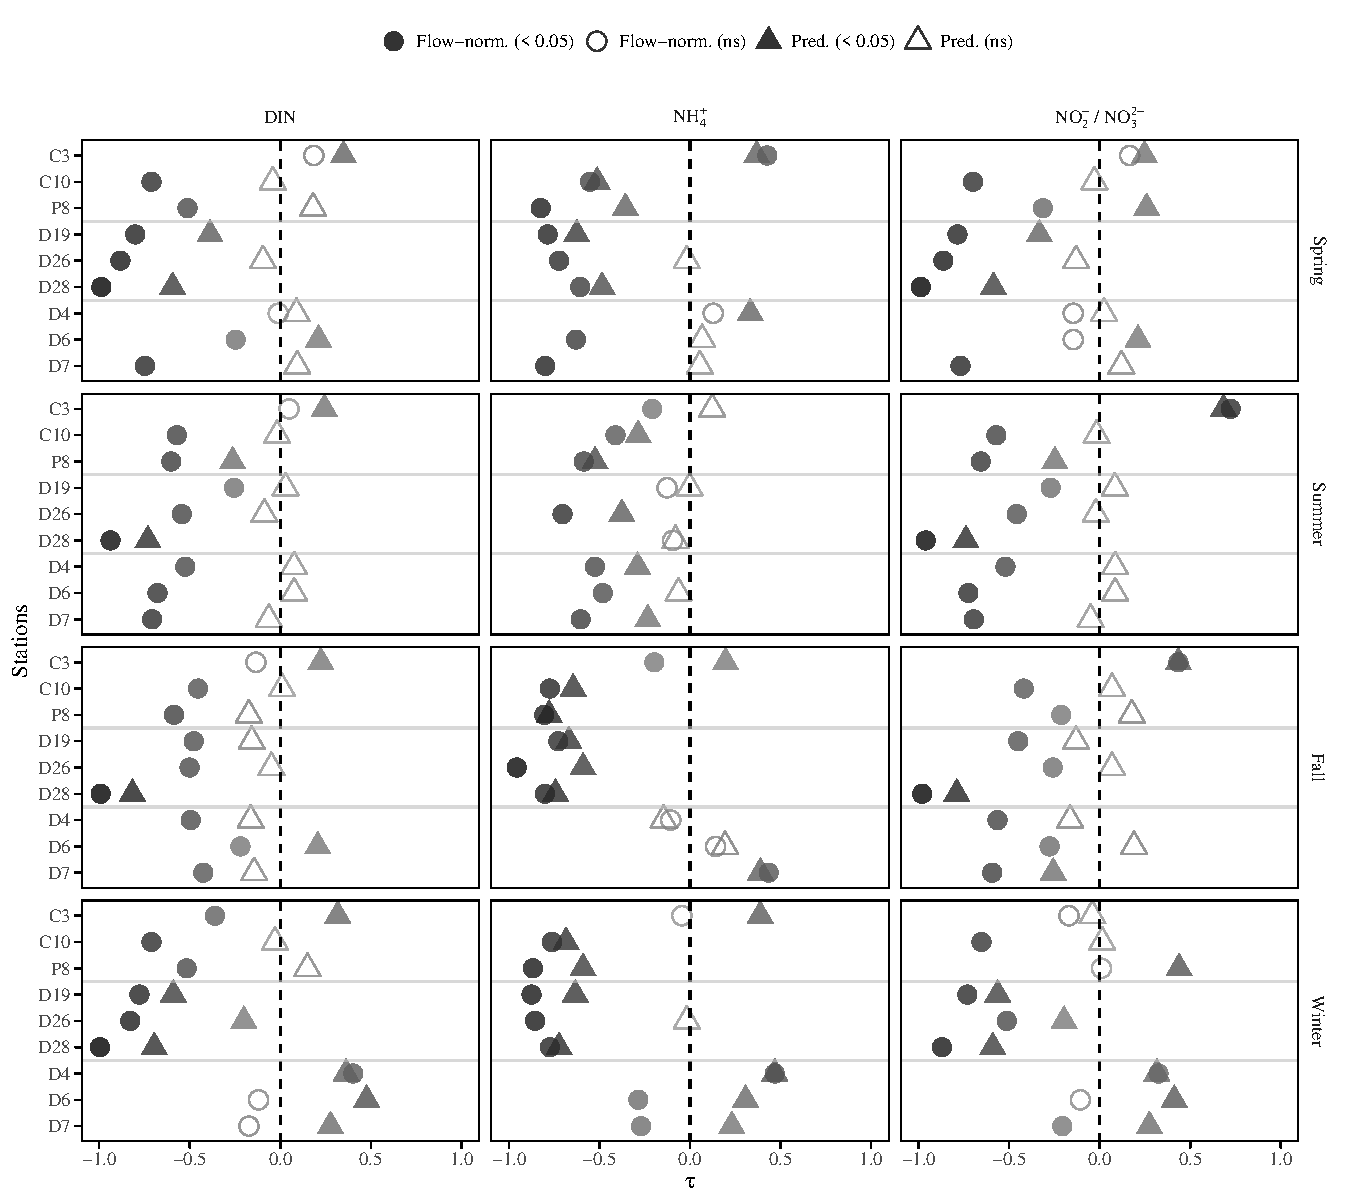
\includegraphics[width=1\textwidth,page=1]{figs/trndcomp3.pdf}
\caption{Results from seasonal Kendall tests on observed data (triangles) and flow-normalized predictions (circles) from \ac{wrtds} for nitrogen analytes. Results are shown as the percent change per year as the estimated Theil-Sen slope divided by the median for a given aggregation period (significance evaluated at $\alpha = 0.05$, based on $\tau$). Trends are shown separately for different seasonal groupings from 1996-2013. Months for each season are Spring: MAM, Summer: JJA, Fall: SON, Winter: DJF. See Figure 3 for annual comparisons.}
\label{fig:trndcomp3}   
\end{figure}

\begin{figure}[!ht]

{\centering 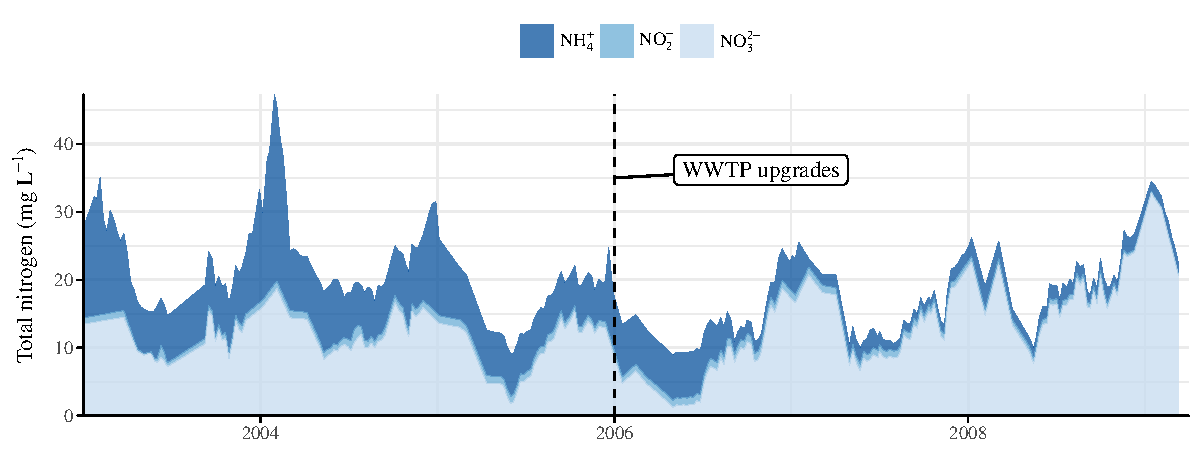
\includegraphics[width=\textwidth]{figs/stock-1} 

}

\caption[Nitrogen concentration measurements (mg L$^{-1}$) from the City of Stockton Wastewater Treatment Plant, San Joaquin County]{Nitrogen concentration measurements (mg L$^{-1}$) from the City of Stockton Wastewater Treatment Plant, San Joaquin County.  Wastewater discharge requirements were implemented in 2006 for nitrification/denitrification and tertiary filtration to convert ammonium to nitrate.}\label{fig:stock}
\end{figure}



\clearpage

% overall trends, years
%latex.default(tab[, -c(1, 2)], file = "", rowlabel = "Analyte/Station",     caption = cap.val, caption.loc = "top", rgroup = vars, n.rgroup = rep(nrow(tab)/3,         3), cgroup = c("Annual"), n.cgroup = c(2), rowname = stats,     label = "tab:trndsann", insert.bottom = foot.val)%
\begin{table}[!tbp]
\caption{Summaries of flow-normalized trends in nitrogen analytes for all stations and annual aggregations.  Summaries are  medians (mg L$^{-1}$) and percent change per year in parentheses (increasing in bold-italic). Changes and significance estimates are based on seasonal Kendall tests of flow-normalized results within each time period.\label{tab:trndsann}} 
\begin{center}
\begin{tabular}{lll}
\hline\hline
\multicolumn{1}{l}{\bfseries Analyte/Station}&\multicolumn{2}{c}{\bfseries Annual}\tabularnewline
\cline{2-3}
\multicolumn{1}{l}{}&\multicolumn{1}{c}{1976-1995}&\multicolumn{1}{c}{1996-2013}\tabularnewline
\hline
{\bfseries DIN}&&\tabularnewline
~~C10&1.3 \footnotesize{(\textit{\textbf{0.8}})**}&1.4 \footnotesize{(-3.1)**}\tabularnewline
~~C3&0.3 \footnotesize{(\textit{\textbf{2.2}})**}&0.5 \footnotesize{(-0.1)**}\tabularnewline
~~D19&0.4 \footnotesize{(\textit{\textbf{0.2}})**}&0.4 \footnotesize{(-1.9)**}\tabularnewline
~~D26&0.4 \footnotesize{(\textit{\textbf{0.4}})**}&0.5 \footnotesize{(-1.2)**}\tabularnewline
~~D28&0.4 \footnotesize{(\textit{\textbf{0.1}})**}&0.4 \footnotesize{(-3.1)**}\tabularnewline
~~D4&0.3 \footnotesize{(\textit{\textbf{0.6}})**}&0.4 \footnotesize{(-0.3)**}\tabularnewline
~~D6&0.4 \footnotesize{(\textit{\textbf{1.8}})**}&0.5 \footnotesize{(-0.3)**}\tabularnewline
~~D7&0.4 \footnotesize{(\textit{\textbf{1.7}})**}&0.5 \footnotesize{(-0.7)**}\tabularnewline
~~MD10&0.4 \footnotesize{(-1.1)**}&0.3 \footnotesize{(-2.4)**}\tabularnewline
~~P8&1.3 \footnotesize{(\textit{\textbf{2.5}})**}&1.7 \footnotesize{(-2)**}\tabularnewline
\hline
{\bfseries NH$_{4}^{+}$}&&\tabularnewline
~~C10&0.1 \footnotesize{(-3.4)**}&0 \footnotesize{(-5.2)**}\tabularnewline
~~C3&0.2 \footnotesize{(\textit{\textbf{3.7}})**}&0.3 \footnotesize{(\textit{\textbf{0}})}\tabularnewline
~~D19&0 \footnotesize{(\textit{\textbf{0.4}})**}&0 \footnotesize{(-1.7)**}\tabularnewline
~~D26&0.1 \footnotesize{(\textit{\textbf{2.2}})**}&0.1 \footnotesize{(-1.5)**}\tabularnewline
~~D28&0 \footnotesize{(-1.1)**}&0 \footnotesize{(-1.4)**}\tabularnewline
~~D4&0 \footnotesize{(\textit{\textbf{0.9}})**}&0.1 \footnotesize{(\textit{\textbf{0}})}\tabularnewline
~~D6&0.1 \footnotesize{(\textit{\textbf{2.4}})**}&0.1 \footnotesize{(-0.5)**}\tabularnewline
~~D7&0.1 \footnotesize{(\textit{\textbf{1.5}})**}&0.1 \footnotesize{(-1.2)**}\tabularnewline
~~MD10&0.1 \footnotesize{(-2.8)**}&0 \footnotesize{(-1.1)**}\tabularnewline
~~P8&0.2 \footnotesize{(\textit{\textbf{4.9}})**}&0.1 \footnotesize{(-10.3)**}\tabularnewline
\hline
{\bfseries NO$_{2}^{-}$/NO$_{3}^{2-}$}&&\tabularnewline
~~C10&1.2 \footnotesize{(\textit{\textbf{1.4}})**}&1.4 \footnotesize{(-3)**}\tabularnewline
~~C3&0.1 \footnotesize{(-0.1)**}&0.2 \footnotesize{(\textit{\textbf{0.7}})**}\tabularnewline
~~D19&0.4 \footnotesize{(-0.1)**}&0.4 \footnotesize{(-1.9)**}\tabularnewline
~~D26&0.3 \footnotesize{(\textit{\textbf{0}})}&0.4 \footnotesize{(-1.1)**}\tabularnewline
~~D28&0.4 \footnotesize{(-0.2)**}&0.4 \footnotesize{(-3.1)**}\tabularnewline
~~D4&0.3 \footnotesize{(\textit{\textbf{0.7}})**}&0.3 \footnotesize{(-0.4)**}\tabularnewline
~~D6&0.3 \footnotesize{(\textit{\textbf{1.3}})**}&0.4 \footnotesize{(-0.3)**}\tabularnewline
~~D7&0.4 \footnotesize{(\textit{\textbf{0.7}})**}&0.4 \footnotesize{(-0.7)**}\tabularnewline
~~MD10&0.4 \footnotesize{(-1)**}&0.3 \footnotesize{(-2.5)**}\tabularnewline
~~P8&1.2 \footnotesize{(\textit{\textbf{1.7}})**}&1.5 \footnotesize{(-0.6)**}\tabularnewline
\hline
\end{tabular}\end{center}

\footnotesize *$p<0.05$; **$p<0.005$\end{table}


% overall trends, seasons, first annual periodyears
%latex.default(tab[, -c(1, 2)], file = "", rowlabel = "Analyte/Station",     caption = cap.val, caption.loc = "top", rgroup = vars, n.rgroup = rep(nrow(tab)/3,         3), cgroup = c("Seasonal, 1976-1995"), n.cgroup = c(4),     rowname = stats, label = "tab:trndsbef", insert.bottom = foot.val)%
\begin{table}[!tbp]
\caption{Summaries of flow-normalized trends in nitrogen analytes for all stations and seasonal aggregations from 1976-1995. Summaries are  medians (mg L$^{-1}$) and percent change per year in parentheses (increasing in bold-italic). Changes and significance estimates are based on seasonal Kendall tests of flow-normalized results within each time period. Months for each season are Spring: MAM, Summer: JJA, Fall: SON, Winter: DJF.\label{tab:trndsbef}} 
\begin{center}
\begin{tabular}{lllll}
\hline\hline
\multicolumn{1}{l}{\bfseries Analyte/Station}&\multicolumn{4}{c}{\bfseries Seasonal, 1976-1995}\tabularnewline
\cline{2-5}
\multicolumn{1}{l}{}&\multicolumn{1}{c}{Spring}&\multicolumn{1}{c}{Summer}&\multicolumn{1}{c}{Fall}&\multicolumn{1}{c}{Winter}\tabularnewline
\hline
{\bfseries DIN}&&&&\tabularnewline
~~C10&1.2 \footnotesize{(\textit{\textbf{1.1}})**}&1.2 \footnotesize{(\textit{\textbf{0.3}})}&1.3 \footnotesize{(\textit{\textbf{0.5}})**}&1.7 \footnotesize{(\textit{\textbf{1.2}})**}\tabularnewline
~~C3&0.3 \footnotesize{(\textit{\textbf{2.4}})**}&0.3 \footnotesize{(\textit{\textbf{2.3}})**}&0.4 \footnotesize{(\textit{\textbf{2.4}})**}&0.4 \footnotesize{(\textit{\textbf{1.9}})**}\tabularnewline
~~D19&0.5 \footnotesize{(\textit{\textbf{0.3}})}&0.2 \footnotesize{(\textit{\textbf{0.4}})}&0.3 \footnotesize{(\textit{\textbf{0.7}})**}&0.7 \footnotesize{(-0.2)}\tabularnewline
~~D26&0.4 \footnotesize{(\textit{\textbf{0.7}})**}&0.3 \footnotesize{(\textit{\textbf{0.4}})*}&0.4 \footnotesize{(\textit{\textbf{1}})**}&0.6 \footnotesize{(\textit{\textbf{0.3}})}\tabularnewline
~~D28&0.5 \footnotesize{(\textit{\textbf{0.8}})*}&0.2 \footnotesize{(\textit{\textbf{0.3}})}&0.3 \footnotesize{(\textit{\textbf{0.5}})*}&0.8 \footnotesize{(-0.3)}\tabularnewline
~~D4&0.4 \footnotesize{(\textit{\textbf{0.2}})}&0.3 \footnotesize{(\textit{\textbf{1.4}})**}&0.3 \footnotesize{(\textit{\textbf{1.1}})**}&0.5 \footnotesize{(-0.5)}\tabularnewline
~~D6&0.4 \footnotesize{(\textit{\textbf{0.4}})}&0.3 \footnotesize{(\textit{\textbf{4.6}})**}&0.4 \footnotesize{(\textit{\textbf{1.4}})**}&0.5 \footnotesize{(-0.7)*}\tabularnewline
~~D7&0.4 \footnotesize{(-0.2)}&0.3 \footnotesize{(\textit{\textbf{4.2}})**}&0.4 \footnotesize{(\textit{\textbf{1.5}})**}&0.6 \footnotesize{(-2.4)**}\tabularnewline
~~MD10&0.6 \footnotesize{(-0.3)}&0.2 \footnotesize{(-3.6)**}&0.3 \footnotesize{(\textit{\textbf{0.8}})**}&1.3 \footnotesize{(-0.3)*}\tabularnewline
~~P8&1.3 \footnotesize{(\textit{\textbf{2.4}})**}&0.9 \footnotesize{(\textit{\textbf{2.4}})**}&1.3 \footnotesize{(\textit{\textbf{3.1}})**}&1.9 \footnotesize{(\textit{\textbf{2.1}})**}\tabularnewline
\hline
{\bfseries NH$_{4}^{+}$}&&&&\tabularnewline
~~C10&0.1 \footnotesize{(-2.3)**}&0 \footnotesize{(-6.8)**}&0.1 \footnotesize{(-7.1)**}&0.3 \footnotesize{(-1.5)**}\tabularnewline
~~C3&0.2 \footnotesize{(\textit{\textbf{3.9}})**}&0.2 \footnotesize{(\textit{\textbf{4}})**}&0.3 \footnotesize{(\textit{\textbf{3.8}})**}&0.2 \footnotesize{(\textit{\textbf{2.9}})**}\tabularnewline
~~D19&0.1 \footnotesize{(\textit{\textbf{0.4}})*}&0 \footnotesize{(-1.7)**}&0 \footnotesize{(\textit{\textbf{1.2}})**}&0.1 \footnotesize{(\textit{\textbf{2.5}})**}\tabularnewline
~~D26&0.1 \footnotesize{(\textit{\textbf{1.4}})**}&0.1 \footnotesize{(\textit{\textbf{2.5}})**}&0.1 \footnotesize{(\textit{\textbf{3.1}})**}&0.1 \footnotesize{(\textit{\textbf{2.3}})**}\tabularnewline
~~D28&0.1 \footnotesize{(-0.5)}&0 \footnotesize{(-3.7)**}&0 \footnotesize{(-1.6)**}&0.1 \footnotesize{(\textit{\textbf{1.7}})**}\tabularnewline
~~D4&0.1 \footnotesize{(\textit{\textbf{1.7}})**}&0 \footnotesize{(\textit{\textbf{1}})**}&0 \footnotesize{(-0.7)}&0.1 \footnotesize{(\textit{\textbf{2}})**}\tabularnewline
~~D6&0.1 \footnotesize{(\textit{\textbf{2.9}})**}&0.1 \footnotesize{(\textit{\textbf{2.8}})**}&0.1 \footnotesize{(-0.1)}&0.1 \footnotesize{(\textit{\textbf{2.1}})**}\tabularnewline
~~D7&0.1 \footnotesize{(\textit{\textbf{3.3}})**}&0 \footnotesize{(\textit{\textbf{2}})**}&0.1 \footnotesize{(-2.8)**}&0.1 \footnotesize{(\textit{\textbf{1.7}})**}\tabularnewline
~~MD10&0.1 \footnotesize{(-1.8)**}&0 \footnotesize{(-6.5)**}&0 \footnotesize{(-3.3)**}&0.2 \footnotesize{(\textit{\textbf{0.4}})}\tabularnewline
~~P8&0.2 \footnotesize{(\textit{\textbf{3.9}})**}&0.1 \footnotesize{(\textit{\textbf{1.8}})**}&0.2 \footnotesize{(\textit{\textbf{7}})**}&0.6 \footnotesize{(\textit{\textbf{7}})**}\tabularnewline
\hline
{\bfseries NO$_{2}^{-}$/NO$_{3}^{2-}$}&&&&\tabularnewline
~~C10&1.1 \footnotesize{(\textit{\textbf{1.5}})**}&1.2 \footnotesize{(\textit{\textbf{0.6}})**}&1.2 \footnotesize{(\textit{\textbf{1.3}})**}&1.5 \footnotesize{(\textit{\textbf{1.8}})**}\tabularnewline
~~C3&0.2 \footnotesize{(\textit{\textbf{0.7}})**}&0.1 \footnotesize{(-1)**}&0.1 \footnotesize{(-0.3)}&0.2 \footnotesize{(\textit{\textbf{1}})**}\tabularnewline
~~D19&0.4 \footnotesize{(\textit{\textbf{0.4}})}&0.2 \footnotesize{(-0.3)}&0.3 \footnotesize{(\textit{\textbf{0.3}})}&0.6 \footnotesize{(-0.9)*}\tabularnewline
~~D26&0.4 \footnotesize{(\textit{\textbf{0.6}})*}&0.2 \footnotesize{(-0.1)}&0.3 \footnotesize{(\textit{\textbf{0.3}})*}&0.5 \footnotesize{(-0.3)}\tabularnewline
~~D28&0.5 \footnotesize{(\textit{\textbf{0.7}})*}&0.2 \footnotesize{(-0.1)}&0.3 \footnotesize{(\textit{\textbf{0.2}})}&0.7 \footnotesize{(-1)**}\tabularnewline
~~D4&0.3 \footnotesize{(\textit{\textbf{0.1}})}&0.3 \footnotesize{(\textit{\textbf{1.4}})**}&0.3 \footnotesize{(\textit{\textbf{1.1}})**}&0.4 \footnotesize{(-0.8)*}\tabularnewline
~~D6&0.4 \footnotesize{(-0.2)}&0.3 \footnotesize{(\textit{\textbf{4.1}})**}&0.3 \footnotesize{(\textit{\textbf{1.4}})**}&0.4 \footnotesize{(-1)**}\tabularnewline
~~D7&0.4 \footnotesize{(-1)*}&0.3 \footnotesize{(\textit{\textbf{3.4}})**}&0.4 \footnotesize{(\textit{\textbf{0.4}})}&0.4 \footnotesize{(-3.6)**}\tabularnewline
~~MD10&0.5 \footnotesize{(-0.2)}&0.2 \footnotesize{(-3.6)**}&0.2 \footnotesize{(\textit{\textbf{1.5}})**}&1.2 \footnotesize{(-0.5)*}\tabularnewline
~~P8&1.2 \footnotesize{(\textit{\textbf{2}})**}&0.9 \footnotesize{(\textit{\textbf{2.3}})**}&1.1 \footnotesize{(\textit{\textbf{2}})**}&1.4 \footnotesize{(\textit{\textbf{1}})**}\tabularnewline
\hline
\end{tabular}\end{center}

\footnotesize *$p<0.05$; **$p<0.005$\end{table}


% overall trends, seasons, first annual periodyears
%latex.default(tab[, -c(1, 2)], file = "", rowlabel = "Analyte/Station",     caption = cap.val, caption.loc = "top", rgroup = vars, n.rgroup = rep(nrow(tab)/3,         3), cgroup = c("Seasonal, 1996-2013"), n.cgroup = c(4),     rowname = stats, label = "tab:trndsaft", insert.bottom = foot.val)%
\begin{table}[!tbp]
\caption{Summaries of flow-normalized trends in nitrogen analytes for all stations and seasonal aggregations from 1996-2013. Summaries are  medians (mg L$^{-1}$) and percent change per year in parentheses (increasing in bold-italic). Changes and significance estimates are based on seasonal Kendall tests of flow-normalized results within each time period. Months for each season are Spring: MAM, Summer: JJA, Fall: SON, Winter: DJF.\label{tab:trndsaft}} 
\begin{center}
\begin{tabular}{lllll}
\hline\hline
\multicolumn{1}{l}{\bfseries Analyte/Station}&\multicolumn{4}{c}{\bfseries Seasonal, 1996-2013}\tabularnewline
\cline{2-5}
\multicolumn{1}{l}{}&\multicolumn{1}{c}{Spring}&\multicolumn{1}{c}{Summer}&\multicolumn{1}{c}{Fall}&\multicolumn{1}{c}{Winter}\tabularnewline
\hline
{\bfseries DIN}&&&&\tabularnewline
~~C10&1.1 \footnotesize{(-4.1)**}&1.3 \footnotesize{(-3.1)**}&1.6 \footnotesize{(-2)**}&1.7 \footnotesize{(-3.4)**}\tabularnewline
~~C3&0.5 \footnotesize{(\textit{\textbf{0.5}})}&0.4 \footnotesize{(\textit{\textbf{0.1}})}&0.6 \footnotesize{(-0.2)}&0.5 \footnotesize{(-0.6)**}\tabularnewline
~~D19&0.5 \footnotesize{(-2.8)**}&0.2 \footnotesize{(-1)*}&0.3 \footnotesize{(-1.6)**}&0.7 \footnotesize{(-2.3)**}\tabularnewline
~~D26&0.5 \footnotesize{(-1.9)**}&0.3 \footnotesize{(-1.7)**}&0.4 \footnotesize{(-1)**}&0.6 \footnotesize{(-0.8)**}\tabularnewline
~~D28&0.5 \footnotesize{(-3)**}&0.2 \footnotesize{(-4.9)**}&0.2 \footnotesize{(-4.9)**}&0.7 \footnotesize{(-2.1)**}\tabularnewline
~~D4&0.4 \footnotesize{(\textit{\textbf{0}})}&0.4 \footnotesize{(-1)**}&0.4 \footnotesize{(-0.9)**}&0.5 \footnotesize{(\textit{\textbf{0.6}})**}\tabularnewline
~~D6&0.5 \footnotesize{(-0.2)*}&0.5 \footnotesize{(-1)**}&0.5 \footnotesize{(-0.3)*}&0.5 \footnotesize{(-0.1)}\tabularnewline
~~D7&0.5 \footnotesize{(-0.8)**}&0.4 \footnotesize{(-1.3)**}&0.4 \footnotesize{(-0.4)**}&0.6 \footnotesize{(-0.2)}\tabularnewline
~~MD10&0.4 \footnotesize{(-2.3)**}&0.2 \footnotesize{(-3.7)**}&0.2 \footnotesize{(-4.4)**}&1 \footnotesize{(-1.8)**}\tabularnewline
~~P8&1.5 \footnotesize{(-1.9)**}&1.2 \footnotesize{(-3.5)**}&1.8 \footnotesize{(-2.4)**}&2.7 \footnotesize{(-2.2)**}\tabularnewline
\hline
{\bfseries NH$_{4}^{+}$}&&&&\tabularnewline
~~C10&0 \footnotesize{(-4.2)**}&0 \footnotesize{(-6.1)**}&0 \footnotesize{(-8.5)**}&0.1 \footnotesize{(-7.3)**}\tabularnewline
~~C3&0.3 \footnotesize{(\textit{\textbf{1}})**}&0.3 \footnotesize{(-0.8)*}&0.4 \footnotesize{(-0.5)*}&0.2 \footnotesize{(-0.1)}\tabularnewline
~~D19&0 \footnotesize{(-1.9)**}&0 \footnotesize{(-0.4)}&0 \footnotesize{(-2.2)**}&0.1 \footnotesize{(-1.8)**}\tabularnewline
~~D26&0.1 \footnotesize{(-1.2)**}&0.1 \footnotesize{(-1.3)**}&0.1 \footnotesize{(-1.9)**}&0.1 \footnotesize{(-1.4)**}\tabularnewline
~~D28&0 \footnotesize{(-1.7)**}&0 \footnotesize{(-0.2)}&0 \footnotesize{(-2.4)**}&0.1 \footnotesize{(-3.1)**}\tabularnewline
~~D4&0.1 \footnotesize{(\textit{\textbf{0.3}})}&0 \footnotesize{(-1.3)**}&0.1 \footnotesize{(-0.3)}&0.1 \footnotesize{(\textit{\textbf{1}})**}\tabularnewline
~~D6&0.1 \footnotesize{(-0.7)**}&0.1 \footnotesize{(-1)**}&0.1 \footnotesize{(\textit{\textbf{0.3}})}&0.1 \footnotesize{(-0.3)**}\tabularnewline
~~D7&0.1 \footnotesize{(-2.2)**}&0 \footnotesize{(-2.1)**}&0.1 \footnotesize{(\textit{\textbf{1.3}})**}&0.1 \footnotesize{(-0.4)*}\tabularnewline
~~MD10&0 \footnotesize{(-1.4)*}&0 \footnotesize{(-0.1)}&0 \footnotesize{(-0.8)**}&0.1 \footnotesize{(-4.3)**}\tabularnewline
~~P8&0.2 \footnotesize{(-8.7)**}&0.1 \footnotesize{(-6.3)**}&0.2 \footnotesize{(-10.4)**}&0.5 \footnotesize{(-13.1)**}\tabularnewline
\hline
{\bfseries NO$_{2}^{-}$/NO$_{3}^{2-}$}&&&&\tabularnewline
~~C10&1.1 \footnotesize{(-4.2)**}&1.2 \footnotesize{(-3.2)**}&1.6 \footnotesize{(-1.9)**}&1.6 \footnotesize{(-3.3)**}\tabularnewline
~~C3&0.2 \footnotesize{(\textit{\textbf{0.4}})}&0.1 \footnotesize{(\textit{\textbf{3.1}})**}&0.2 \footnotesize{(\textit{\textbf{1.7}})**}&0.2 \footnotesize{(-0.4)}\tabularnewline
~~D19&0.4 \footnotesize{(-2.9)**}&0.2 \footnotesize{(-1)*}&0.3 \footnotesize{(-1.5)**}&0.6 \footnotesize{(-2.2)**}\tabularnewline
~~D26&0.4 \footnotesize{(-1.9)**}&0.2 \footnotesize{(-1.6)**}&0.3 \footnotesize{(-0.6)*}&0.5 \footnotesize{(-0.6)**}\tabularnewline
~~D28&0.5 \footnotesize{(-3)**}&0.2 \footnotesize{(-5.4)**}&0.2 \footnotesize{(-5.2)**}&0.7 \footnotesize{(-1.7)**}\tabularnewline
~~D4&0.3 \footnotesize{(-0.1)}&0.3 \footnotesize{(-1)**}&0.3 \footnotesize{(-1)**}&0.4 \footnotesize{(\textit{\textbf{0.4}})**}\tabularnewline
~~D6&0.4 \footnotesize{(-0.1)}&0.4 \footnotesize{(-1)**}&0.4 \footnotesize{(-0.4)*}&0.4 \footnotesize{(-0.1)}\tabularnewline
~~D7&0.4 \footnotesize{(-0.6)**}&0.4 \footnotesize{(-1.2)**}&0.4 \footnotesize{(-0.8)**}&0.4 \footnotesize{(-0.3)*}\tabularnewline
~~MD10&0.4 \footnotesize{(-2.6)**}&0.1 \footnotesize{(-4.5)**}&0.2 \footnotesize{(-5.4)**}&1 \footnotesize{(-1.4)**}\tabularnewline
~~P8&1.3 \footnotesize{(-1.1)**}&1.1 \footnotesize{(-3.1)**}&1.6 \footnotesize{(-0.3)*}&2.2 \footnotesize{(\textit{\textbf{0}})}\tabularnewline
\hline
\end{tabular}\end{center}

\footnotesize *$p<0.05$; **$p<0.005$\end{table}


\end{document}
